\subsection{Cosmic Radiation Methods}
\label{sec:Rad-Methods}

\subsection{Telemetry}
\label{sec:Telemetry}

All telemetry was handled via the RPi. The DB9 interface from the HASP Large Payload plate was converted to a 
RS-232 female plug. A Male RS 232 to Male USB \ref{fig:rs232-usb} was used to connect it to a USB port of the RPi. 
The downlink data packets were written to describe the radiation data. 
The uplink commands were sent to the RPi which delegated the work either to itself or the Arduino which 
was connected to the RPi via USB as shown in figure \ref{fig:telem-diagram}.

\begin{figure}[h!]
\centering
\begin{minipage}{.5\textwidth}
  \centering
  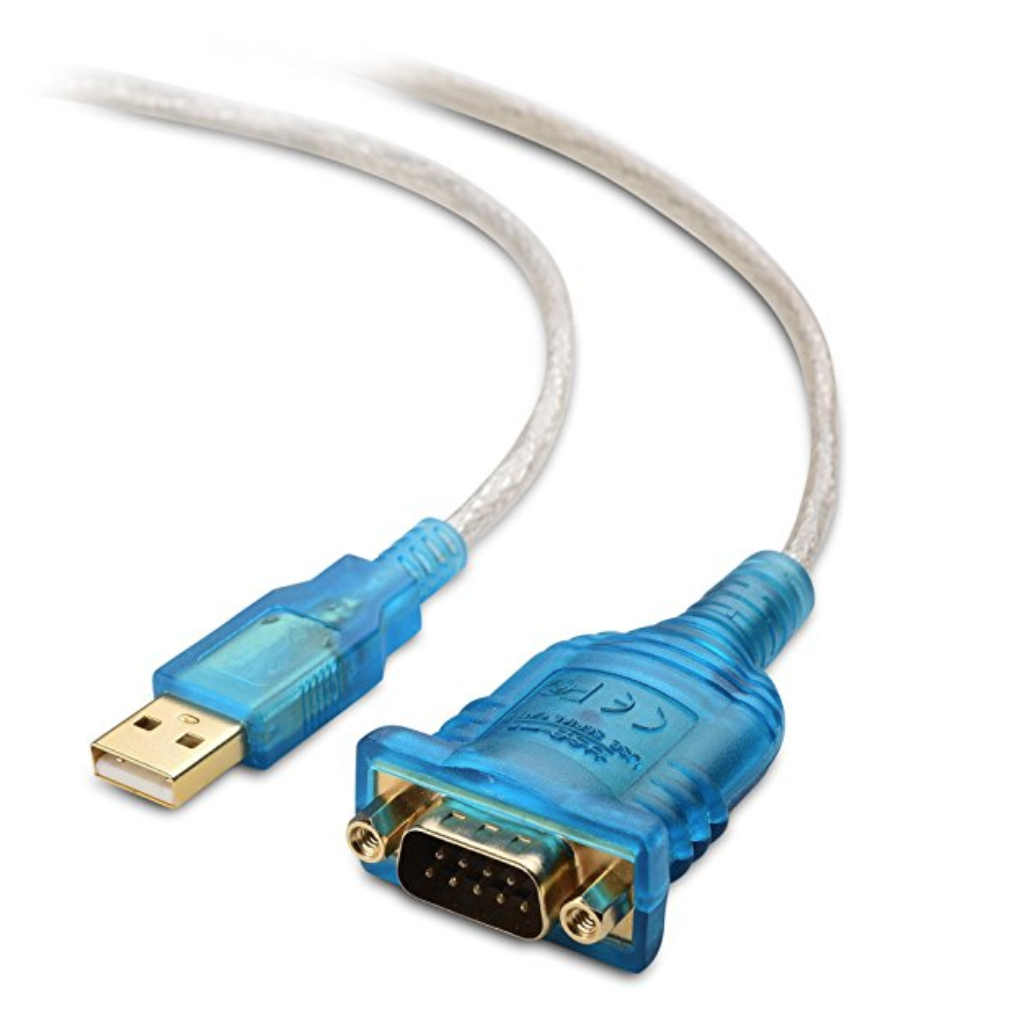
\includegraphics[width=.4\linewidth]{figures/rs232tousb.png}
  \caption{RS 232 to Male USB}{Cable used to connect the DB9 interface to the RPi}
  \label{fig:rs232tousb}
\end{minipage}%
\begin{minipage}{.5\textwidth}
  \centering
  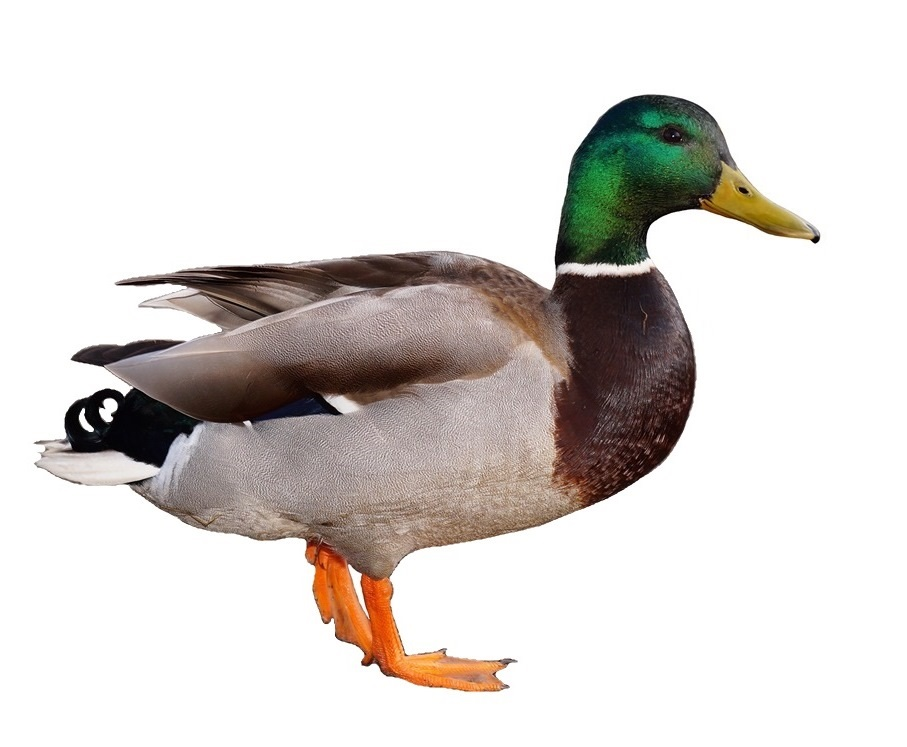
\includegraphics[width=.4\linewidth]{figures/duck.jpg}
  \caption{Telemetry}{Diagram depicting how telemetry was processed}
  \label{fig:telem-diagram}
\end{minipage}
\end{figure}

\subsubsection{Uplink}
\label{sec:Uplink} 
Uplink commands were used to start, end, and change parameters within our payload over the course of flight. 
Table \ref{table:Commands} list the uplink commands, thier functions and a brief description of what they did. 

\subsubsection{Downlink}
\label{sec:Downlink}
Downlink data was written to describe the data being read from the MiniPix detector. 

\begin{table}[h!]
\centering
\caption{Table of All Uplink Commands Used During Flight}
\label{tab:All-Commands}
\bigskip
\begin{tabular}{c|c|c|c}
\hline
\hline
\multicolumn{1}{c|}{\bfseries Command} & \multicolumn{1}{c|}{\bfseries Byte 1} &  \multicolumn{1}{c|}{\bfseries Byte 2} & \multicolumn{1}{c}{\bfseries Expected Current Consumption} \\
\hline
    	Start Acquisition  	& 0x01	& -	 		& \SI{0.47}{\ampere}    \\ \hline
    	End Acquistion 		& 0x02	& -	 		& \SI{0.29}{\ampere}    \\ \hline
    	Change Shutter Rate 	& 0x03 	& 0x01 to 0xFF *	& nominal A 		\\ \hline
	Change Acquisition Mode	& 0x04	& 0x01 or 0x02 **	& nominal A		\\ \hline
	Astrobiology System On	& 0x05	& -			& spike			\\ \hline
	Astrobiology System Off	& 0x06	& -			& nominal		\\ \hline
\begin{tablenotes}* This parameter denotes the new shutter rate in seconds the MiniPix detector would begin to take acquistions}
\end{tabular}
\medskip
\end{table}

Below is a sample of real data packets recieved during flight. 

\lstset{basicstyle=\small, numbers=left, xleftmargin=2em, frame=tb, label = Downlinks, framexleftmargin=1.5em}
\begin{lstlisting}[caption = Sample of downlinked data packets ID: 15667 - 15670.]
...
some samples here
...
\end{lstlisting}
